\documentclass[a4paper,10pt]{article}
\usepackage[utf8]{inputenc}
\usepackage[]{polski}
\usepackage{a4wide}
\usepackage{caption}
\usepackage{float}
\usepackage{amsthm}
\usepackage{graphicx}

\title{{\textbf{Pracownia z analizy numerycznej}}\\[1ex]
       {\Large Sprawozdanie do zadania \textbf{P2.20.}}\\[-1ex]
       {\Large Redukcja macierzy metodą Gaussa}\\
       {\large Prowadzący: dr Witold Karczewski}}
\author{Aleksander Balicki, \large nr indeksu: 220989\\
	Dominika Rogozińska, \large nr indeksu: 221094}

% Kropka po numerze paragrafu, podparagrafu itp. 
\makeatletter
	\renewcommand\@seccntformat[1]{\csname the#1\endcsname.\quad}
	\renewcommand\numberline[1]{#1.\hskip0.7em}
\makeatother

% Kropka po numerze tablicy, rysunku i ustawienie czcionki dla etykiety. 
\captionsetup{labelfont=sc,labelsep=period}

% Numeracja wzorów według paragrafu.
\renewcommand{\theequation}{\arabic{section}.\arabic{subsection}.\arabic{equation}}

% Zmiana nazwy figure "Rysunek" -> "Wykres"
\renewcommand{\figurename}{Wykres}

% Środowisko definition z numeracją
\newtheorem{definition}{Definicja}
\newtheorem{theorem}{Twierdzenie}


\date{Wrocław, \today r.}
\begin{document}
\maketitle

\section{Wstęp}
\setcounter{equation}{0}
Metodę Gaussa redukcji macierzy wykorzystuje się do rozwiązywania takich problemów jak znajdowanie macierzy odwrotnej, obliczanie rzędu macierzy, a także rozwiązywanie układów równań z wieloma niewiadomymi. Efektywność tej metody zależy od szczegółów implementacji i modyfikacji algorytmu oraz wskaźnika uwarunkowania macierzy. Poniżej zostały zaprezentowane wyniki otrzymane dla eliminacji Gaussa bez i z następującymi modyfikacjami: wybór największego(co do modułu) reduktora z wiersza, z kolumny, z podmacierzy(wybór pełny). Badania zostały przeprowadzone dla kilku rodzajów macierzy: macierzy Hilberta, macierzy Pei, macierzy losowej z dominującą przekątną oraz macierzy oraz macierzy losowej, w ktorej większość elementów należy do przedziału $(-1,1)$, a kilka jest wybranych z zakresu $(-1000,1000)$.

\section{Definicje}
\begin{definition}
	Macierzą o wymiarach $m \times n$ (macierzą o $m$ wierszach i $n$ kolumnach), nad ciałem $K$ nazywamy każdą funkcję typu $\{1,\cdots,m\} \times \{1,\cdots,n\} \rightarrow K$.
\end{definition}
Interesują będą nas macierze o rozmiarach $n \times n$, które przedstawiają układy $n$ równań z $n$ niewiadomymi. Przykładowymi danymi do badań sposobów rozwiązania takich układów były macierze rzędu $n$, które są nieosobliwe, więc układy te zawsze mają rozwiązanie.
Macierz zapisujemy w następujący sposób:
\begin{center}
	$ \left[ \begin{array}{cccc}
		a_{1,1} & a_{1,2} & \cdots & a_{1,n}\\
		a_{2,1} & a_{2,2} & \cdots & a_{2,n}\\
		\vdots  &  \vdots &        & \vdots \\
		a_{m,1} & a_{m,2} & \cdots & a_{m,n}\\
	\end{array} \right] $
\end{center}
\newpage
Weźmy przykładowy układ równań:
\begin{center}
$ \left \{ \begin{array}{ccccccccc}
		a_{1,1}x_{1} & + & a_{1,2}x_{2} & + & \cdots & + & a_{1,n}x_{n} & = & b_{1}\\
		a_{2,1}x_{1} & + & a_{2,2}x_{2} & + & \cdots & + & a_{2,n}x_{n} & = & b_{2}\\
		\vdots & & \vdots & &  \vdots & & \vdots & & \vdots \\
		a_{n,1}x_{1} & + & a_{n,2}x_{2} & + & \cdots & + & a_{n,n}x_{n} & = & b_{n}\\
       \end{array} \right. $
\end{center}
Z tym układem wiążemy macierz układu $A$ oraz wektor wyrazów wolnych $b$:
\begin{center}
$A = \left[ \begin{array}{ccccccccc}
		a_{1,1} & a_{1,2} & \cdots & a_{1,n}\\
		a_{2,1} & a_{2,2} & \cdots & a_{2,n}\\
		\vdots  &  \vdots &        & \vdots \\
		a_{n,1} & a_{n,2} & \cdots & a_{n,n}\\
       \end{array} \right] $
$b = \left[ \begin{array}{c}
		b_{1}\\
		b_{2}\\
		\vdots\\
		b_{n}\\
       \end{array} \right] $
\end{center}

\begin{definition}
	Macierzą Hilberta nazywamy macierz $n \times n$, w której\\
    \begin{center}
    $a_{i,j} = \frac{1}{i+j-1}$
    \end{center}
\end{definition} 

\begin{definition}
	Macierzą Pei nazywamy macierz $n \times n$, w której\\
  \[
  a_{i,j} = \left\{
  \begin{array}{l l}
    1 \quad \texttt{ $i$ $\neq$ $j$ }\\
    d \quad \texttt{ $i$ $=$ $j$ }\\
  \end{array} \right.
  \]
    gdzie $d$ jest parametrem.
\end{definition}

\begin{definition}
    Macierzą o dominującej przekątnej nazywamy macierz, w której\\
    \begin{center}
    $\displaystyle \bigwedge_{1 \leq i \leq n } \sum_{ j \neq i } |a_{i,j}| \leq |a_{i,i}| $
    \end{center}
\end{definition}

\begin{definition}
    Wskaźnik uwarunkowania macierzy $A$ w równaniu $Ax = b$ jest charakterystyczną własnością macierzy, informującą o tym jaki będzie maksymalny stosunek błędu względnego wektora rozwiązania $x$ do błędu względego $b$.
\end{definition}

\begin{definition}
    Normę maksimum dla wektora $x = \left[ x_{1}, x_{2}, \cdots , x_{n} \right] $ definiujemy jako\\
    \begin{center}
        $ \|x\|_{\infty} = max \{|x_{i}| : i = 1, 2, \cdots , n \}$
    \end{center}
\end{definition}

Normy maksimum użyjemy jako wskaźnika numerycznej poprawności metody Gaussa,
porównując wartości $ \| b - A \tilde{x} \|_{\infty}$ dla wszystkich prób.
Wartość $\tilde x$ to nasze przybliżone rozwiązanie, więc $\| b - A \tilde{x} \|_{\infty}$ oznacza największy spośród błędów przybliżeń $x_i$.

\begin{definition}
    Wskaźnik uwarunkowania macierzy $A$ w równaniu $Ax = b$ jest charakterystyczną własnością macierzy, informującą o tym jaki będzie maksymalny stosunek błędu względnego wektora rozwiązania $x$ do błędu względego $b$.
    \begin{center}
        $ \kappa(A) = \|A^{-1}\| \cdot \|A\|$
    \end{center}
    Definicja ta jest taka sama dla każdej zwartej normy.
\end{definition}
\newpage
\section{Metoda eliminacji Gaussa}
Metoda ta została stworzona przez Carla Friedricha Gaussa. Daje ona algorytm do rozwiązania układu równań liniowych,
obliczenia rzędu macierzy i znalezienia macierzy odwrotnej do danej. Algorytm składa się z 2 kroków, najpierw doprowadzamy
macierz do postaci schodkowej, a następnie znajdujemy wynik układu poprzez podstawienie w tył(funkcja back substitution).
W metodzie Gaussa stososuje się 3 operacje elementarne na wierszach macierzy. Te operacje to:
\begin{enumerate}
	\item Zamiana kolejności wierszy
	\item Pomnożenie wszystkich wartości w wierszu przez niezerowy skalar $\lambda$
	\item Dodanie do dowolnego wiersza kombinacji liniowej pozostałych wierszy
\end{enumerate}
Operacje elementarne mają ciekawe własności, mianowicie:
\begin{itemize}
	\item Nie zmieniają rzędu macierzy
	\item Dowolną macierz można za pomocą skończonej liczby kroków doprowadzić do macierzy w postaci schodkowej
\end{itemize}
\subsection{Metoda eliminacji Gaussa bez wyboru elementów głównych}
Wykonujemy następujący algorytm:
\begin{verbatim}
        for k from 1 to N
                przeskaluj k-ty wiersz, aby m[k,k] = 1
                for i from k+1 to N
                        odejmij od i-tego wiersza k-ty wiersz m[i,k] razy
        wykonaj back_substitution
\end{verbatim}
Powyższy algorytm ma pewien problem. Co się stanie, jeżeli $m[k,k] = 0$ dla któregoś $k$? Nie jesteśmy wtedy w stanie
znaleźć takiego skalaru, aby po pomnożeniu na tym miejscu znalazło się $1$. Nawet jeżeli odrzucimy te przypadki,
to na przekątnej mogą się znaleźć elementy bardzo bliskie zeru. Wtedy cały nasz wiersz zostanie podzielony przez
liczbę bliską zeru i wygeneruje duże błędy.

\subsection{Metoda eliminacji Gaussa z wyborem elementów głownych z wiersza lub kolumny}
Jednym sposobem poradzenia sobie z tym problemem jest wybór elementów głównych z wiersza lub kolumny.
W wyborze głównego elementu z wiersza, w każdym kroku głównej pętli naszego programu wyszukujemy maksymalny element
z wiersza i zamieniamy kolumny obecną i tą z maksymalnym elementem. Wiemy, że zamiana kolumn przestawia nam tylko
kolejność zmiennych w rozwiązaniu. Tym sposobem zapewniamy to, że zawsze dzielimy przez największy element z wiersza,
czyli dzielenie przez liczby bliskie zeru występuje rzadziej. Analogicznie działa wybór głównego elementu z kolumny.
\begin{verbatim}
        for k from 1 to N
                znajdz maksymalną wartość |m[k,i]| dla wszystkich i > k
                zamień kolumnę z maksymalną wartością z k-tą kolumną
                przeskaluj k-ty wiersz, aby m[k,k] = 1
                for i from k+1 to N
                        odejmij od i-tego wiersza k-ty wiersz m[i,k] razy
        wykonaj back_substitution
\end{verbatim}

\subsection{Metoda eliminacji Gaussa z pełnym wyborem elementów głównych(z podmacierzy)}
Jest to rozszerzenie poprzedniego pomysłu z wyborem elementów, tym razem wyszukujemy maksymalnego elementu z podmacierzy i 
dokonujemy zamiany wiersza oraz kolumny. Metoda ta jest kosztowna obliczeniowo, bo w każdym kroku musimy znaleść maksymalny
element spośród $O(n^2)$ elementów.

\begin{verbatim}
        for k from 1 to N-1
                znajdz i,l takie, że |m[i,l]| jest maksymalne dla wszystkich i > k, l > k
                zamień l-tą kolumnę z k-tą kolumną
                zamień i-ty wiersze z k-tym wierszem
                przeskaluj k-ty wiersz, aby m[k,k] = 1
                for i from k+1 to N
                        odejmij od i-tego wiersza k-ty wiersz m[i,k] razy
        wykonaj back_substitution1
\end{verbatim}

\section{Program}
	Program testujący jest napisany w języku C++. Użyto typu podwójnej precyzji (double). Wyniki zostały zapisane jako plik z rozszerzeniem .csv, a następnie opracowane graficznie za pomocą programu gnuplot.
	
\section{Wyniki prób}
    \subsection{Macierz Hilberta}
        \begin{center}
            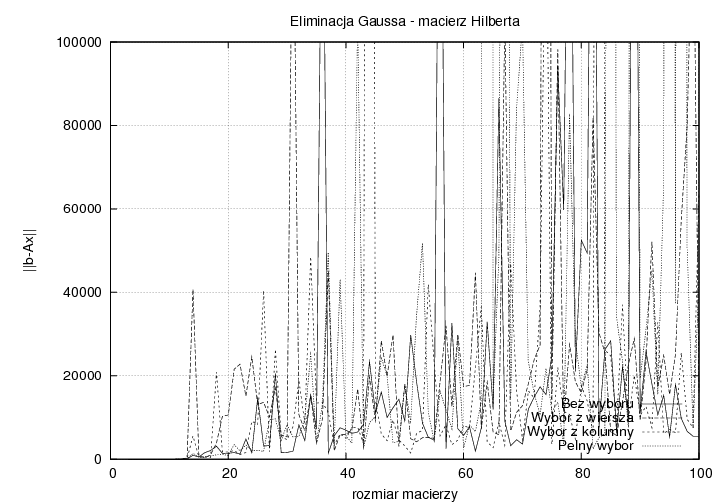
\includegraphics[width=140mm]{hilbert_plot.png}
        \end{center}
        Wskaźnik uwarunkowania macierzy Hilberta o rozmiarze $n$ to\cite{Wi}:
        \begin{center}
            $ \kappa(H_{n}) = O(\frac{e^{3.5255n}}{\sqrt{n}})$
        \end{center}
            Nawet dla małych wartości $n$ wskaźnik uwarunkowania tej macierzy jest zbyt duży, aby dane mogły być reprezentatywne. Powyższy wykres nie prezentuje całego zakresu danych, które wygenerował program.
    \subsection{Macierz Pei}
        \begin{center}
            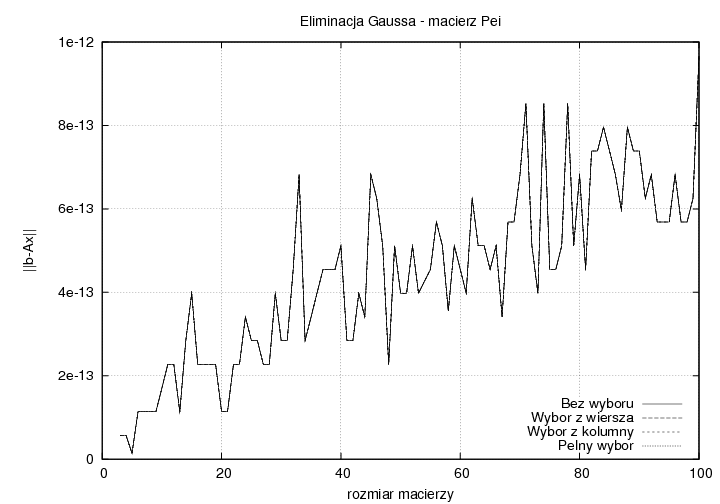
\includegraphics[width=140mm]{pei_plot.png}
        \end{center}
            Macierz Pei jest postaci:\\
        \\
        $P_{n} = \left[ \begin{array}{ccccccccc}
	    d & 1 & \cdots & 1\\
	    1 & d & \cdots & 1\\
	    \vdots & \vdots & & \vdots \\
	    1 & 1 & \cdots & d\\
       \end{array} \right] $\\
        \\
            Macierz odwrotna do macierzy Pei to \cite{Wa}: \\
        \\
        $P_{n}^{-1} = \frac{1}{(d-1)(d+n-1)} \left[ \begin{array}{ccccccccc}
	    d+n-2 & -1 & \cdots & -1\\
	    -1 & d+n-2 & \cdots & -1\\
	    \vdots & \vdots & & \vdots \\
	    -1 & -1 & \cdots & d+n-2\\
       \end{array} \right] $\\
        \\
            Obliczmy wskaźnik uwarunkowania macierzy Pei(użyjemy normy maksymalnej):
        \begin{center}
            $ \kappa(P_{n}) = \|P_{n}^{-1}\|_{\infty} \cdot \|P_{n}\|_{\infty} = |\frac{d+n-2}{(d-1)(d+n-1)}| \cdot |d| = |\frac{d^2+dn-2d}{d^2+dn-2d+1-n}| \approx 1 $
        \end{center}
            Macierz Pei ma dobry wskaźnik uwarunkowania. Wartości zaburzeń przedstawionych na wykresie są nieduże. Wykresy funkcji przedstawiających błędy dla poszczególnych modyfikacji metody Gaussa pokrywają się. Dzieje się tak dlatego, że macierz ta ma na swojej przekątnej liczby $d$, które są większe od pozostałych wartości($1$) w wierszu i takie same, jak największe wartości w pozostałych wierszach. Algorytm Gaussa - z modyfikacjami czy bez - zawsze będzie wybierał jako $\lambda_{k}$ element $a_{k,k}$ dla wiersza $k$.
            Dla $d \geq n$ macierz Pei będzie szczególnym przypadkiem macierzy dominującej przekątniowo.

    \subsection{Macierz z dominującą przekątną}
        \begin{center}
            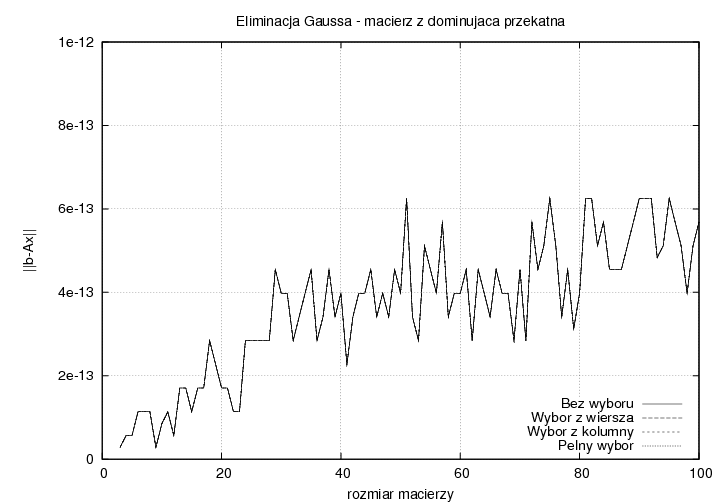
\includegraphics[width=140mm]{dominating_plot.png}
        \end{center}
        Macierz dominująca przekątniowo jest macierzą, dla której możemy bezpiecznie zastosować metodę Gaussa bez wyboru elementów głównych, ponieważ takie elementy już znajdują się na przekątnej. wykresy funkcji prezentujące różne rodzaje metody Gaussa praktycznie się pokrywają - różnice między dokładnością rozwiązań są niewielkie. W tabeli 1. zostały przedstawione wyniki dla niektórych prób.
        \begin{center}
            \begin{tabular}{ | l | l | l | l | l | }
            \hline
            Rozmiar & Gauss & Gauss z wyb. z kolumny & Gauss z wyb. z wiersza & Gauss z pełnym wyborem \\ \hline
            19 & $0.2273 \cdot 10^{-12}$ & $0.2273 \cdot 10^{-12}$ & $0.2273 \cdot 10^{-12}$ & $0.1136 \cdot 10^{-12}$ \\ \hline
            22 & $0.1136 \cdot 10^{-12}$ & $0.1136 \cdot 10^{-12}$ & $0.1136 \cdot 10^{-12}$ & $0.2842 \cdot 10^{-12}$ \\ \hline
            31 & $0.3979 \cdot 10^{-12}$ & $0.3979 \cdot 10^{-12}$ & $0.3979 \cdot 10^{-12}$ & $0.3410 \cdot 10^{-12}$ \\ \hline
            38 & $0.4547 \cdot 10^{-12}$ & $0.4547 \cdot 10^{-12}$ & $0.4547 \cdot 10^{-12}$ & $0.2842 \cdot 10^{-12}$ \\ \hline
            \end{tabular}
        \end{center}
        Możemy zauważyć, że jedynym zauważalnie różniącym się wynikiem jest wartość błędu dla eliminacji Gaussa z pełnym wyborem elementów głównych. Różnica ta nie jest jednak znacząco duża.
    \subsection{Macierz losowa}
        Na wykresie zostały przedstawione funkcje błędu obliczeń od rozmiaru macierzy. Funkcje te nie są monotoniczne - jest to spowodowane faktem, że do każdej próby losowane są inne dane.
        \begin{center}
            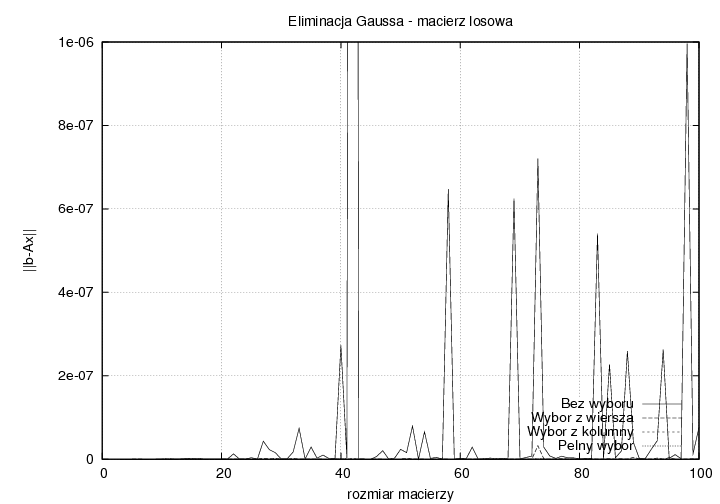
\includegraphics[width=140mm]{random_plot.png}
        \end{center}
        Na wykresie obejmującym cały przedział określoności funkcji nie widać wyraźnej różnicy pomiędzy różnymi modyfikacjami metody Gaussa. Przyjrzyjmy się przybliżeniu tego wykresu:
        \begin{center}
            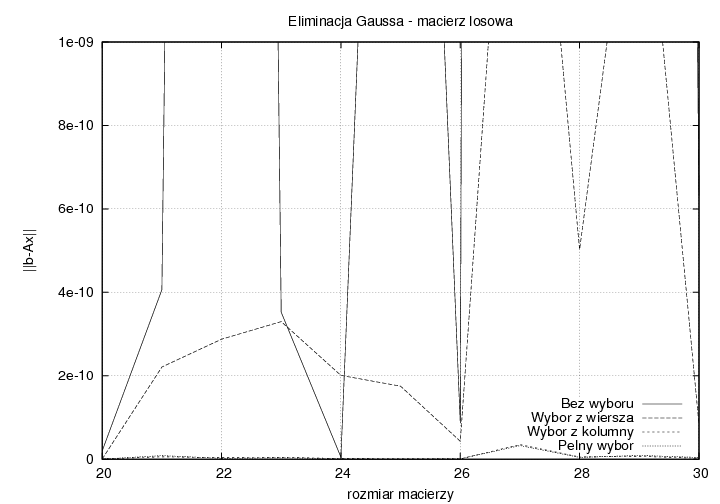
\includegraphics[width=140mm]{random_focus_plot.png}
        \end{center}
        Spoglądając na ten wykres możemy zauważyć, że otrzymujemy lepsze wyniki dla wyboru pełnego i wyboru z kulomny(po którym zamieniamy wiersze) - wyniki dla tych dwóch metod różnią się tylko nieznacznie.\\
    Na wykresach zostały przedstawione tylko dane, dla których podczas eliminacji Gaussa bez wyboru elementów głównych nie było sytuacji, w której na przekątnej macierzy znajduje się $0$.


\section{Wnioski}
    Nie powinniśmy stosować metody eliminacji Gaussa bez wyboru elementów głównych, ponieważ nie zabezpiecza ona przed sytuacją, gdy na głównej przekątnej macierzy pojawi się $0$.
    Metoda Gaussa z pełnym wyborem elementów głównych co prawda daje najlepsze wyniki, jednak ma większą złożoność obliczeniową($(O(n^2)$), a poprawa wyników nie jest na tyle duża, aby warto było ją stosować.
    Metody Gaussa z wyborem z kulumny lub wiersza wydają się dawać najlepsze wyniki, będące kompromisem pomiędzy złożonością algorytmu, a jego numeryczną poprawnością.

	
\begin{thebibliography}{9}
	\bibitem{EK} Notatki z wykładu Algebra Emanuela Kierońskiego
	\bibitem{SL} Notatki z wykładu Analiza Numeryczna Stanisława Lewanowicza
	\bibitem{KC} Kincaid David, Cheney Ward, Analiza numeryczna
	\bibitem{JJ} J. M. Jankowscy, Przegląd metod i algorytmów numerycznych
	\bibitem{Wa} http://wolframalpha.com/
	\bibitem{Wi} http://en.wikipedia.org/
	\bibitem{Mi} http://wazniak.mimuw.edu.pl/
\end{thebibliography}
\end{document}

